%% =========================================================================
\section{Exercise 3: Connection to an Infinite Bus}
%% =========================================================================

Generator~A is replaced by an ideal three-phase voltage source representing an
\textbf{infinite bus} --- a bus that maintains constant terminal voltage and
constant frequency regardless of the active or reactive power exchanged with
it. This models a large national power grid to which a small generator is
connected. By definition, the infinite bus has zero impedance ($Z_\infty
\rightarrow 0$) and infinite apparent power capacity ($S_\infty \rightarrow
\infty$).

The fundamental consequence is that the infinite bus completely dominates
frequency: no action of Generator~B can alter the system frequency.
Generator~B must adapt entirely to the grid's frequency, not the other way
around.

%% ── SIMULINK MODEL DIAGRAM ───────────────────────────────────────────────
\subsection{Simulink Model}

\figref{fig:ex3_diagram} shows the Exercise~3 Simulink model. Generator~A
has been replaced by an ideal three-phase voltage source (infinite bus) that
maintains constant voltage at \pu{1.0} and constant frequency at \Hz{60}.
Generator~B connects through the synchronisation breaker at $t=\SI{5}{s}$.
The infinite bus absorbs or supplies any real and reactive power demanded by
Gen~B without any change in its terminal conditions.

\begin{figure}[H]
  \centering
  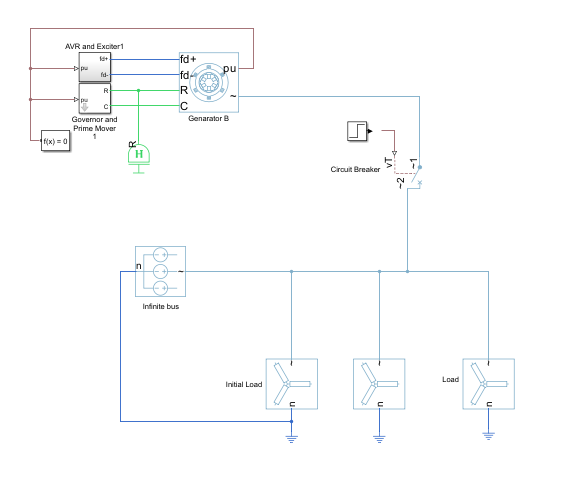
\includegraphics[width=\textwidth]{figures/EX3_diagram.png}
  \caption{Exercise 3 Simulink model: Generator~B connected to an infinite bus
    (ideal voltage source) through a synchronisation breaker. The infinite bus
    maintains $V = \pu{1.0}$ and $f = \Hz{60}$ at all times.}
  \label{fig:ex3_diagram}
\end{figure}

%% ── TASK 5 ────────────────────────────────────────────────────────────────
\subsection{Task 5 -- Generator B at Lower Frequency (0.98\,pu) vs Infinite Bus}

\begin{figure}[H]
  \centering
  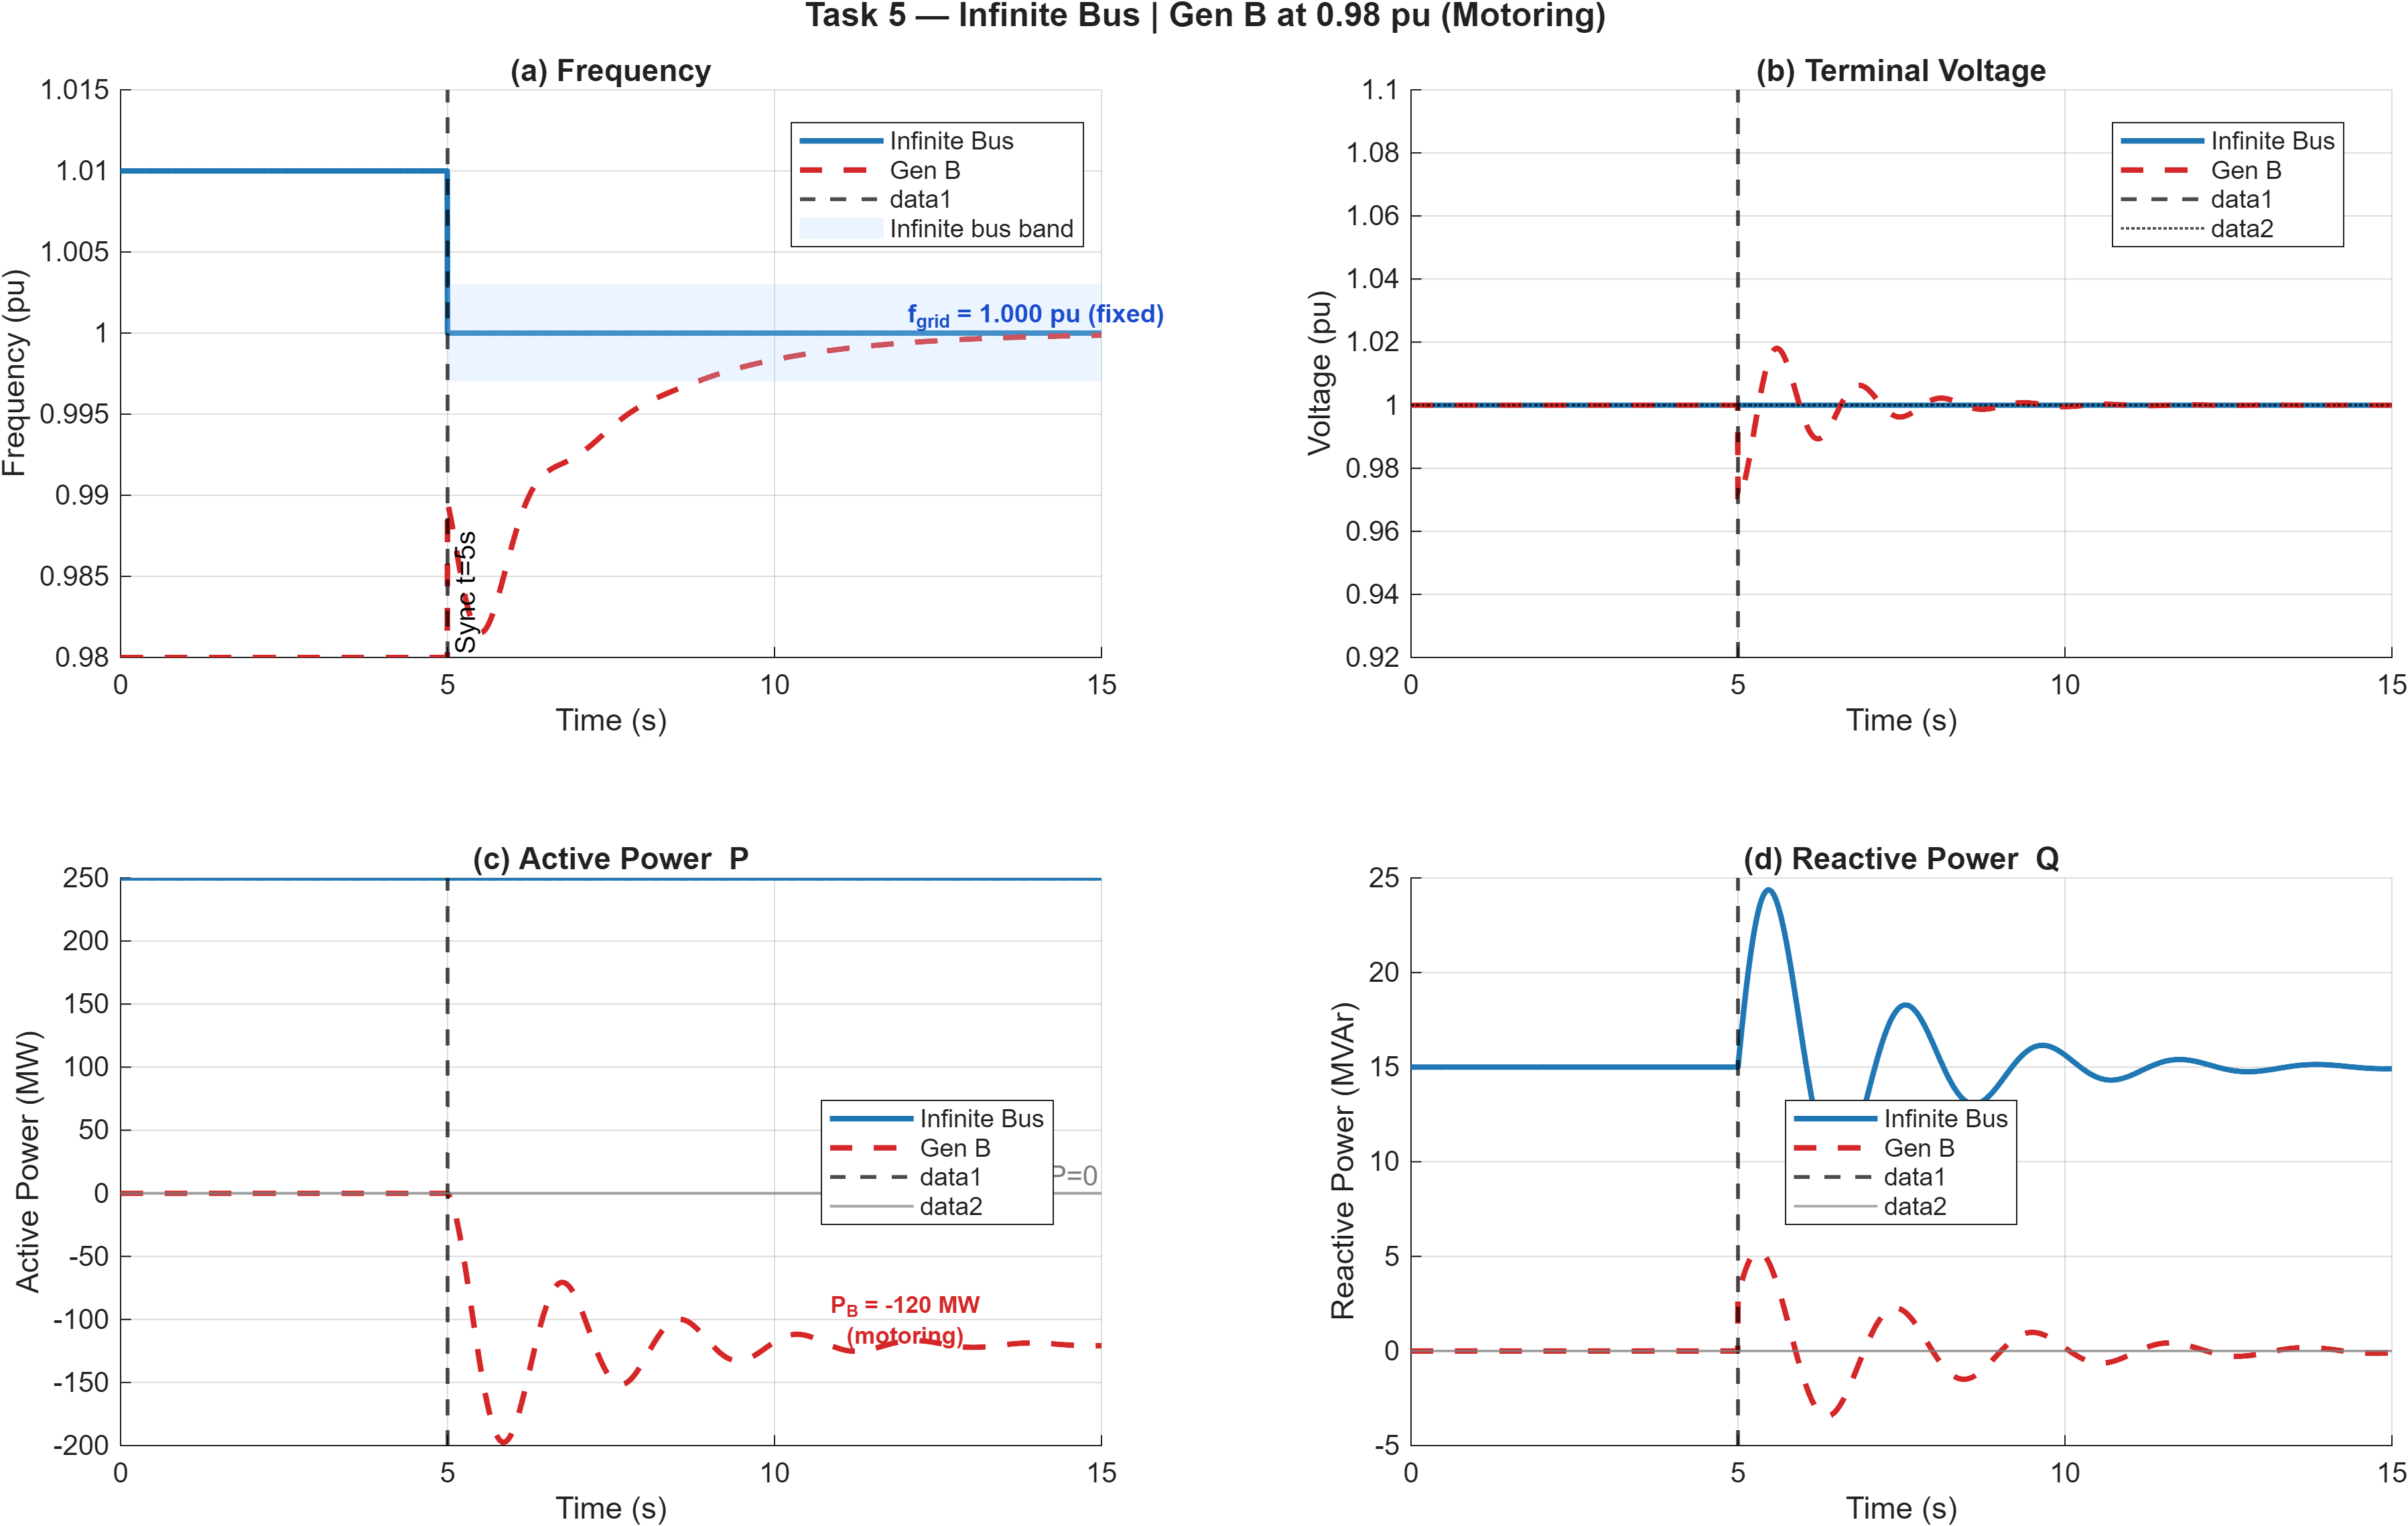
\includegraphics[width=\textwidth]{figures/Task5_AllPlots.png}
  \caption{Task 5: Generator~B paralleled with an infinite bus at
    $f_\text{set} = \pu{0.98}$. System frequency is completely rigid at
    \pu{1.000}. Panels show frequency, terminal voltage, active power, and
    reactive power.}
  \label{fig:task5_all}
\end{figure}

\subsubsection{Frequency (Task 5)}

Upon breaker closure at $t=\SI{5}{s}$, the infinite bus instantaneously
forces Gen~B's frequency to \pu{1.0}. The system frequency does not change
at all --- it remains exactly \pu{1.0} throughout. This is the defining
characteristic of an infinite bus and the fundamental contrast with Task~3.

\subsubsection{Active Power (Task 5)}

With the grid frequency fixed at \pu{1.0} and Gen~B's setpoint at \pu{0.98},
the droop equation gives:

\begin{equation}
  P_B = \frac{f_\text{setpoint} - f_\text{grid}}{S_P}
  = \frac{0.98 - 1.0}{S_P} < 0
  \label{eq:task5_PB}
\end{equation}

Generator~B operates as a synchronous motor, absorbing power from the infinite
bus. This motoring condition is \textit{more severe} than Task~3 because, in
Task~3, the system frequency settled at a compromise value ($\approx\pu{1.008}$),
reducing the setpoint deficit from 0.030 to only 0.028\,pu. Here, the
infinite bus maintains exactly \pu{1.0}, so the full 0.020\,pu deficit drives
a stronger motoring condition.

\subsubsection{Comparison with Task 3}

\tabref{tab:t3_vs_t5} quantifies the contrast between the two scenarios.

\begin{table}[H]
  \centering
  \caption{Task 3 vs Task 5 -- Finite Bus vs Infinite Bus ($f_\text{set,B} = \pu{0.98}$)}
  \label{tab:t3_vs_t5}
  \begin{tabular}{>{\bfseries}p{3.2cm} p{5cm} p{5cm}}
    \toprule
    \textbf{Parameter}
      & \textbf{Task 3 (Finite Bus)}
      & \textbf{Task 5 (Infinite Bus)} \\
    \midrule
    System frequency after sync
      & $\approx\pu{1.008}$ (compromise between setpoints)
      & $\pu{1.000}$ exactly (rigid, unchanged) \\[4pt]
    Gen~B active power
      & Slightly negative (weak motoring)
      & Strongly negative (severe motoring) \\[4pt]
    Freq.\ influence of Gen~B
      & Drags system freq.\ down partially
      & Zero influence on system freq. \\[4pt]
    Voltage regulation
      & Both AVRs act to restore \pu{1.0}
      & Grid holds voltage; AVR acts on Gen~B only \\[4pt]
    Physical analogy
      & Two rubber bands pulling each other
      & Rubber band vs a rigid wall \\[4pt]
    Engineering implication
      & Overloads Gen~A; unstable if repeated
      & Gen~B trips on overload; must raise setpoint \\
    \bottomrule
  \end{tabular}
\end{table}

%% ── TASK 6 ────────────────────────────────────────────────────────────────
\subsection{Task 6 -- Generator B at Higher Frequency (1.01\,pu) vs Infinite Bus}

\begin{figure}[H]
  \centering
  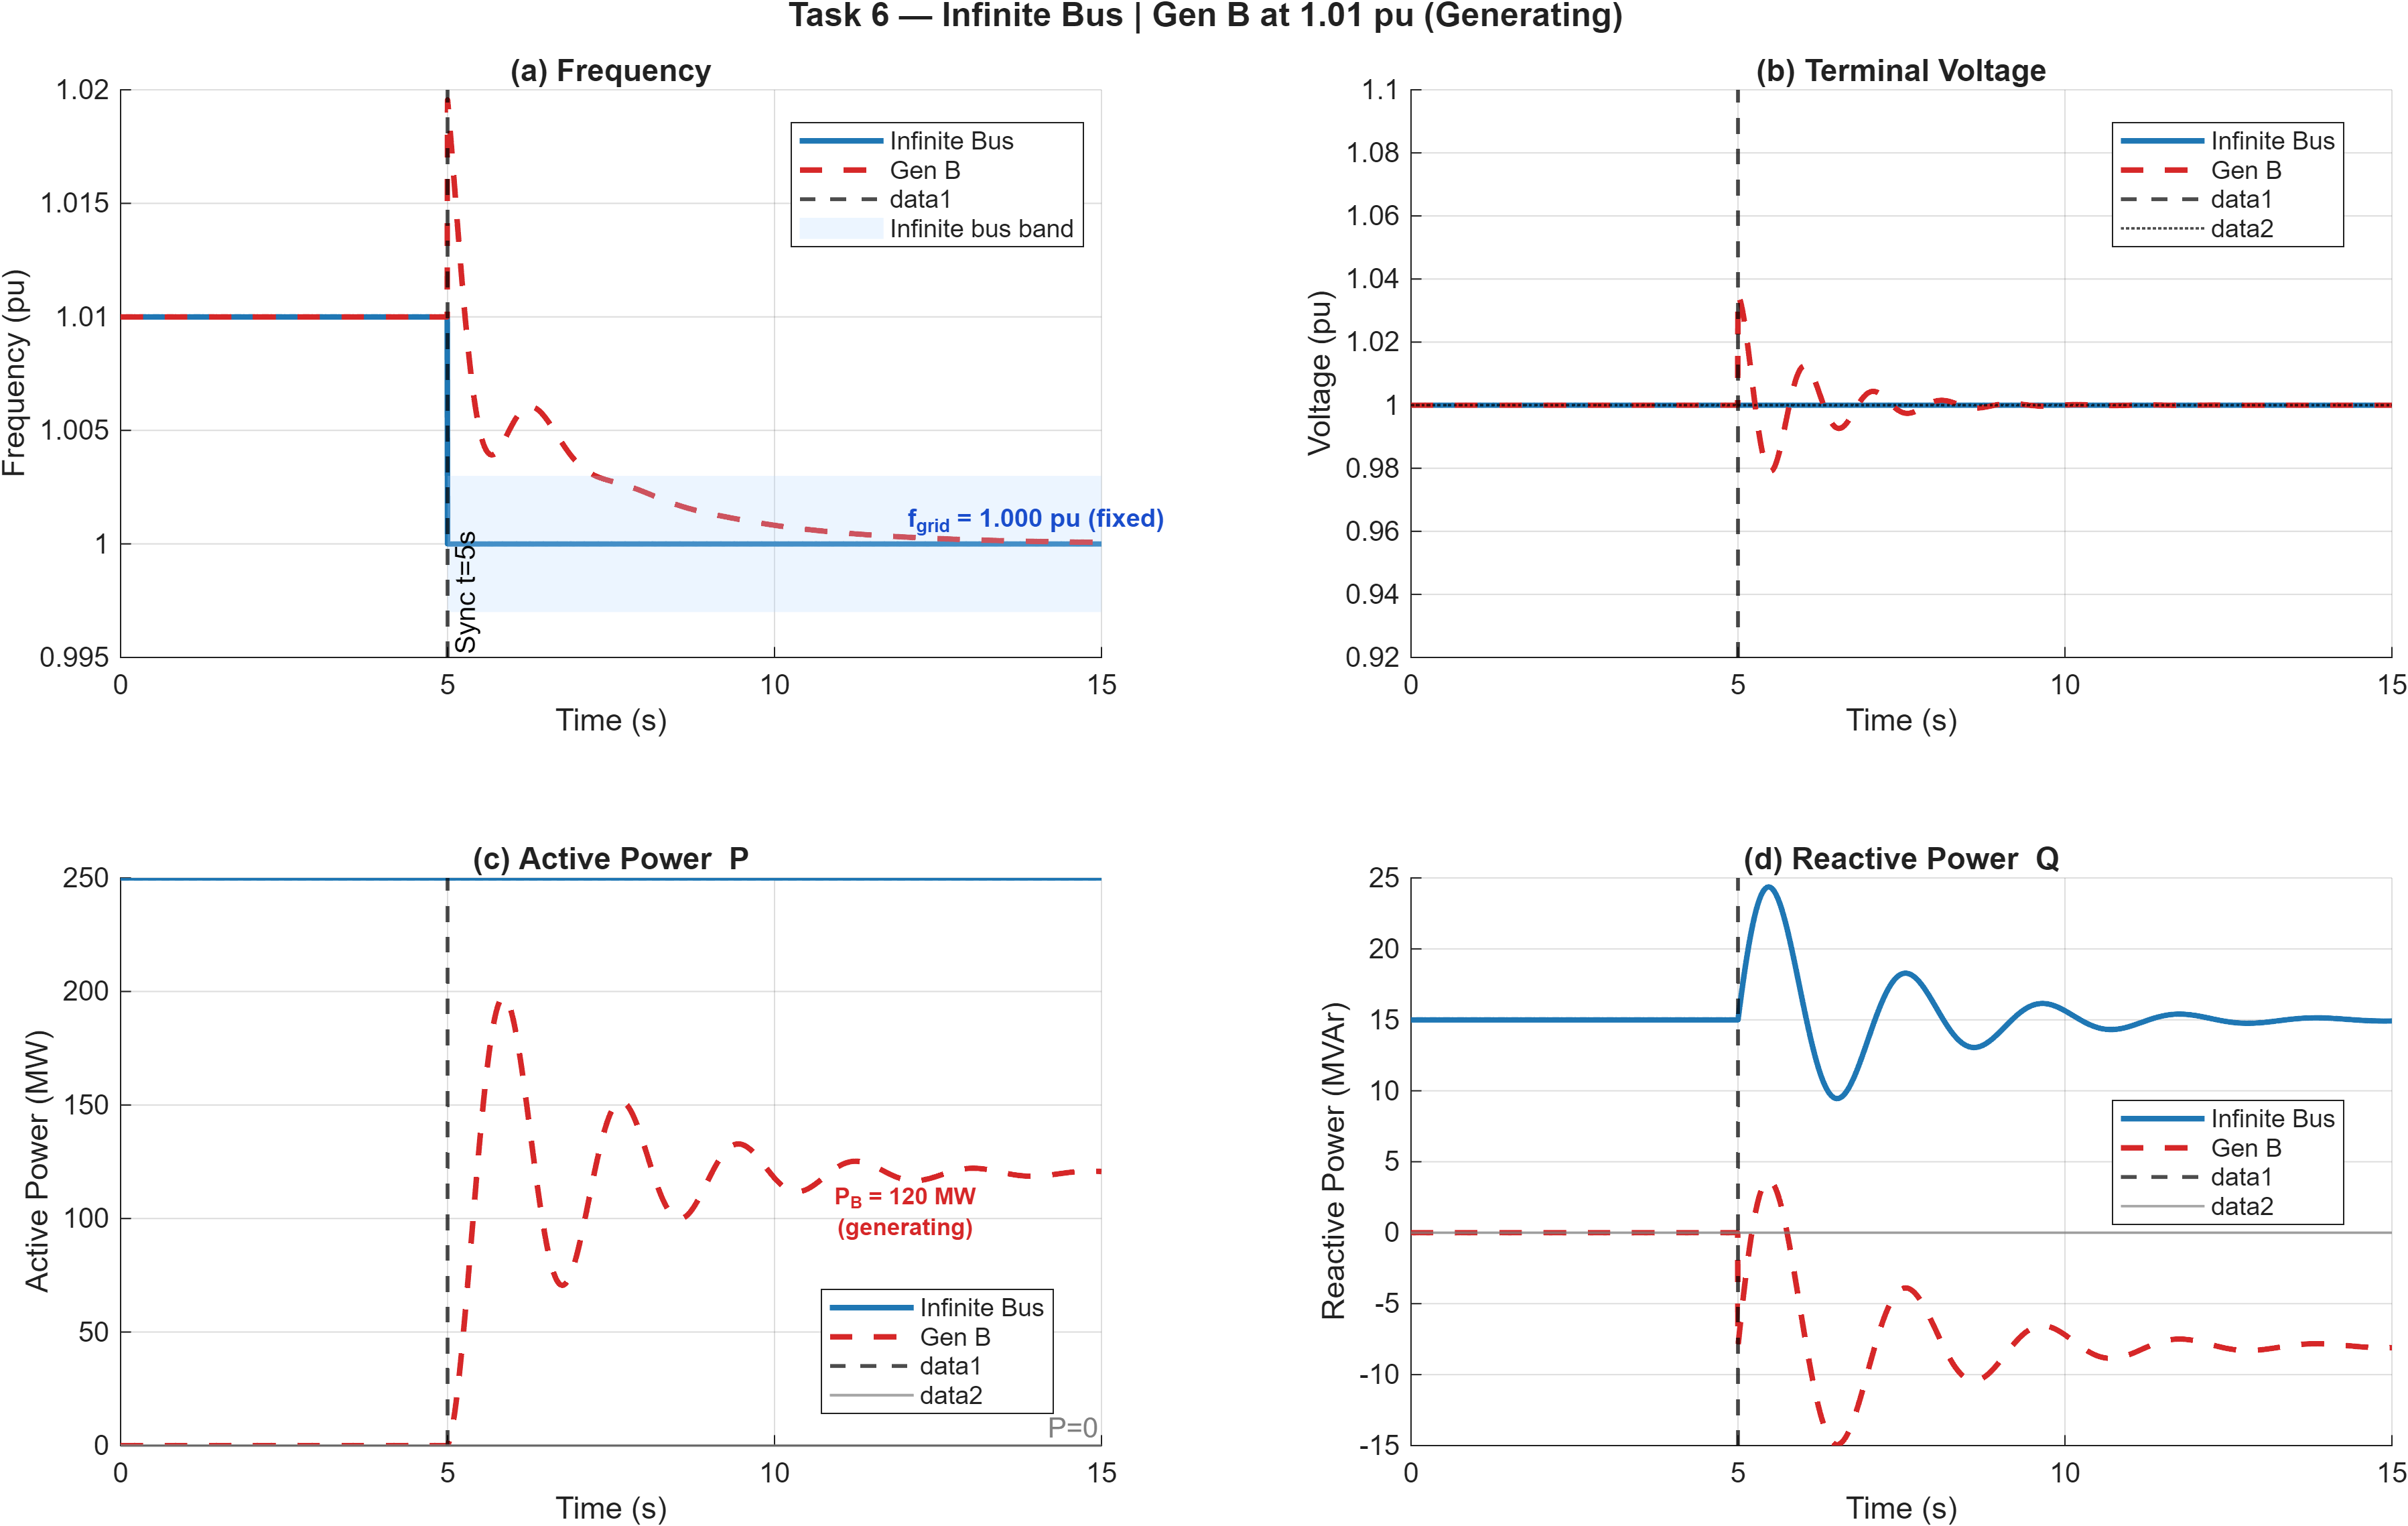
\includegraphics[width=\textwidth]{figures/Task6_AllPlots.png}
  \caption{Task 6: Generator~B paralleled with an infinite bus at
    $f_\text{set} = \pu{1.01}$. System frequency remains rigid at \pu{1.000}.
    Panels show frequency, terminal voltage, active power, and reactive power.}
  \label{fig:task6_all}
\end{figure}

\subsubsection{Frequency (Task 6)}

Generator~B is spun up to \pu{1.01} before synchronisation. Upon breaker
closure, the infinite bus immediately locks Gen~B to \pu{1.0}. The frequency
does not rise --- it remains exactly \pu{1.0}. This is the key contrast with
Task~4, where Gen~A (a finite machine) was pulled upward in frequency by Gen~B,
resulting in a settled system frequency of $\approx\pu{1.023}$.

\subsubsection{Active Power (Task 6)}

With Gen~B's setpoint above the infinite bus frequency:

\begin{equation}
  P_B = \frac{f_\text{setpoint} - f_\text{grid}}{S_P}
  = \frac{1.01 - 1.0}{S_P} > 0
  \label{eq:task6_PB}
\end{equation}

Generator~B injects positive active power into the infinite bus. The grid
absorbs this power effortlessly without any frequency perturbation. After the
synchronisation transient, Gen~B supplies approximately \MW{120} to the grid
in steady state.

\subsubsection{Comparison with Task 4}

\tabref{tab:t4_vs_t6} quantifies the contrast.

\begin{table}[H]
  \centering
  \caption{Task 4 vs Task 6 -- Finite Bus vs Infinite Bus ($f_\text{set,B} = \pu{1.01}$)}
  \label{tab:t4_vs_t6}
  \begin{tabular}{>{\bfseries}p{3.2cm} p{5cm} p{5cm}}
    \toprule
    \textbf{Parameter}
      & \textbf{Task 4 (Finite Bus)}
      & \textbf{Task 6 (Infinite Bus)} \\
    \midrule
    System frequency after sync
      & $\approx\pu{1.023}$ (raised by Gen~B)
      & $\pu{1.000}$ exactly (cannot be raised) \\[4pt]
    Gen~A / Grid response
      & Gen~A reduces output significantly
      & Grid absorbs all Gen~B output silently \\[4pt]
    Gen~B active power
      & $\approx\MW{150}$ (majority of load)
      & $\approx\MW{120}$ (fixed by setpoint) \\[4pt]
    Voltage behaviour
      & Spike then \pu{1.0}
      & Spike then \pu{1.0} (identical mechanism) \\[4pt]
    Freq.\ influence of Gen~B
      & Raises system frequency
      & Cannot raise grid frequency \\[4pt]
    Engineering implication
      & Load transferred; useful commissioning
      & Normal grid-tie generation; power sold \\
    \bottomrule
  \end{tabular}
\end{table}

%% ── GRAND COMPARISON ─────────────────────────────────────────────────────
\subsection{Grand Comparison -- All Tasks}

\figref{fig:grand_comparison} presents the grand comparison across all four
parallel-operation tasks (Tasks~3--6), enabling simultaneous visual assessment
of how the bus type (finite vs infinite) and the governor setpoint (under-frequency
vs over-frequency) interact to determine system behaviour.

\begin{figure}[H]
  \centering
  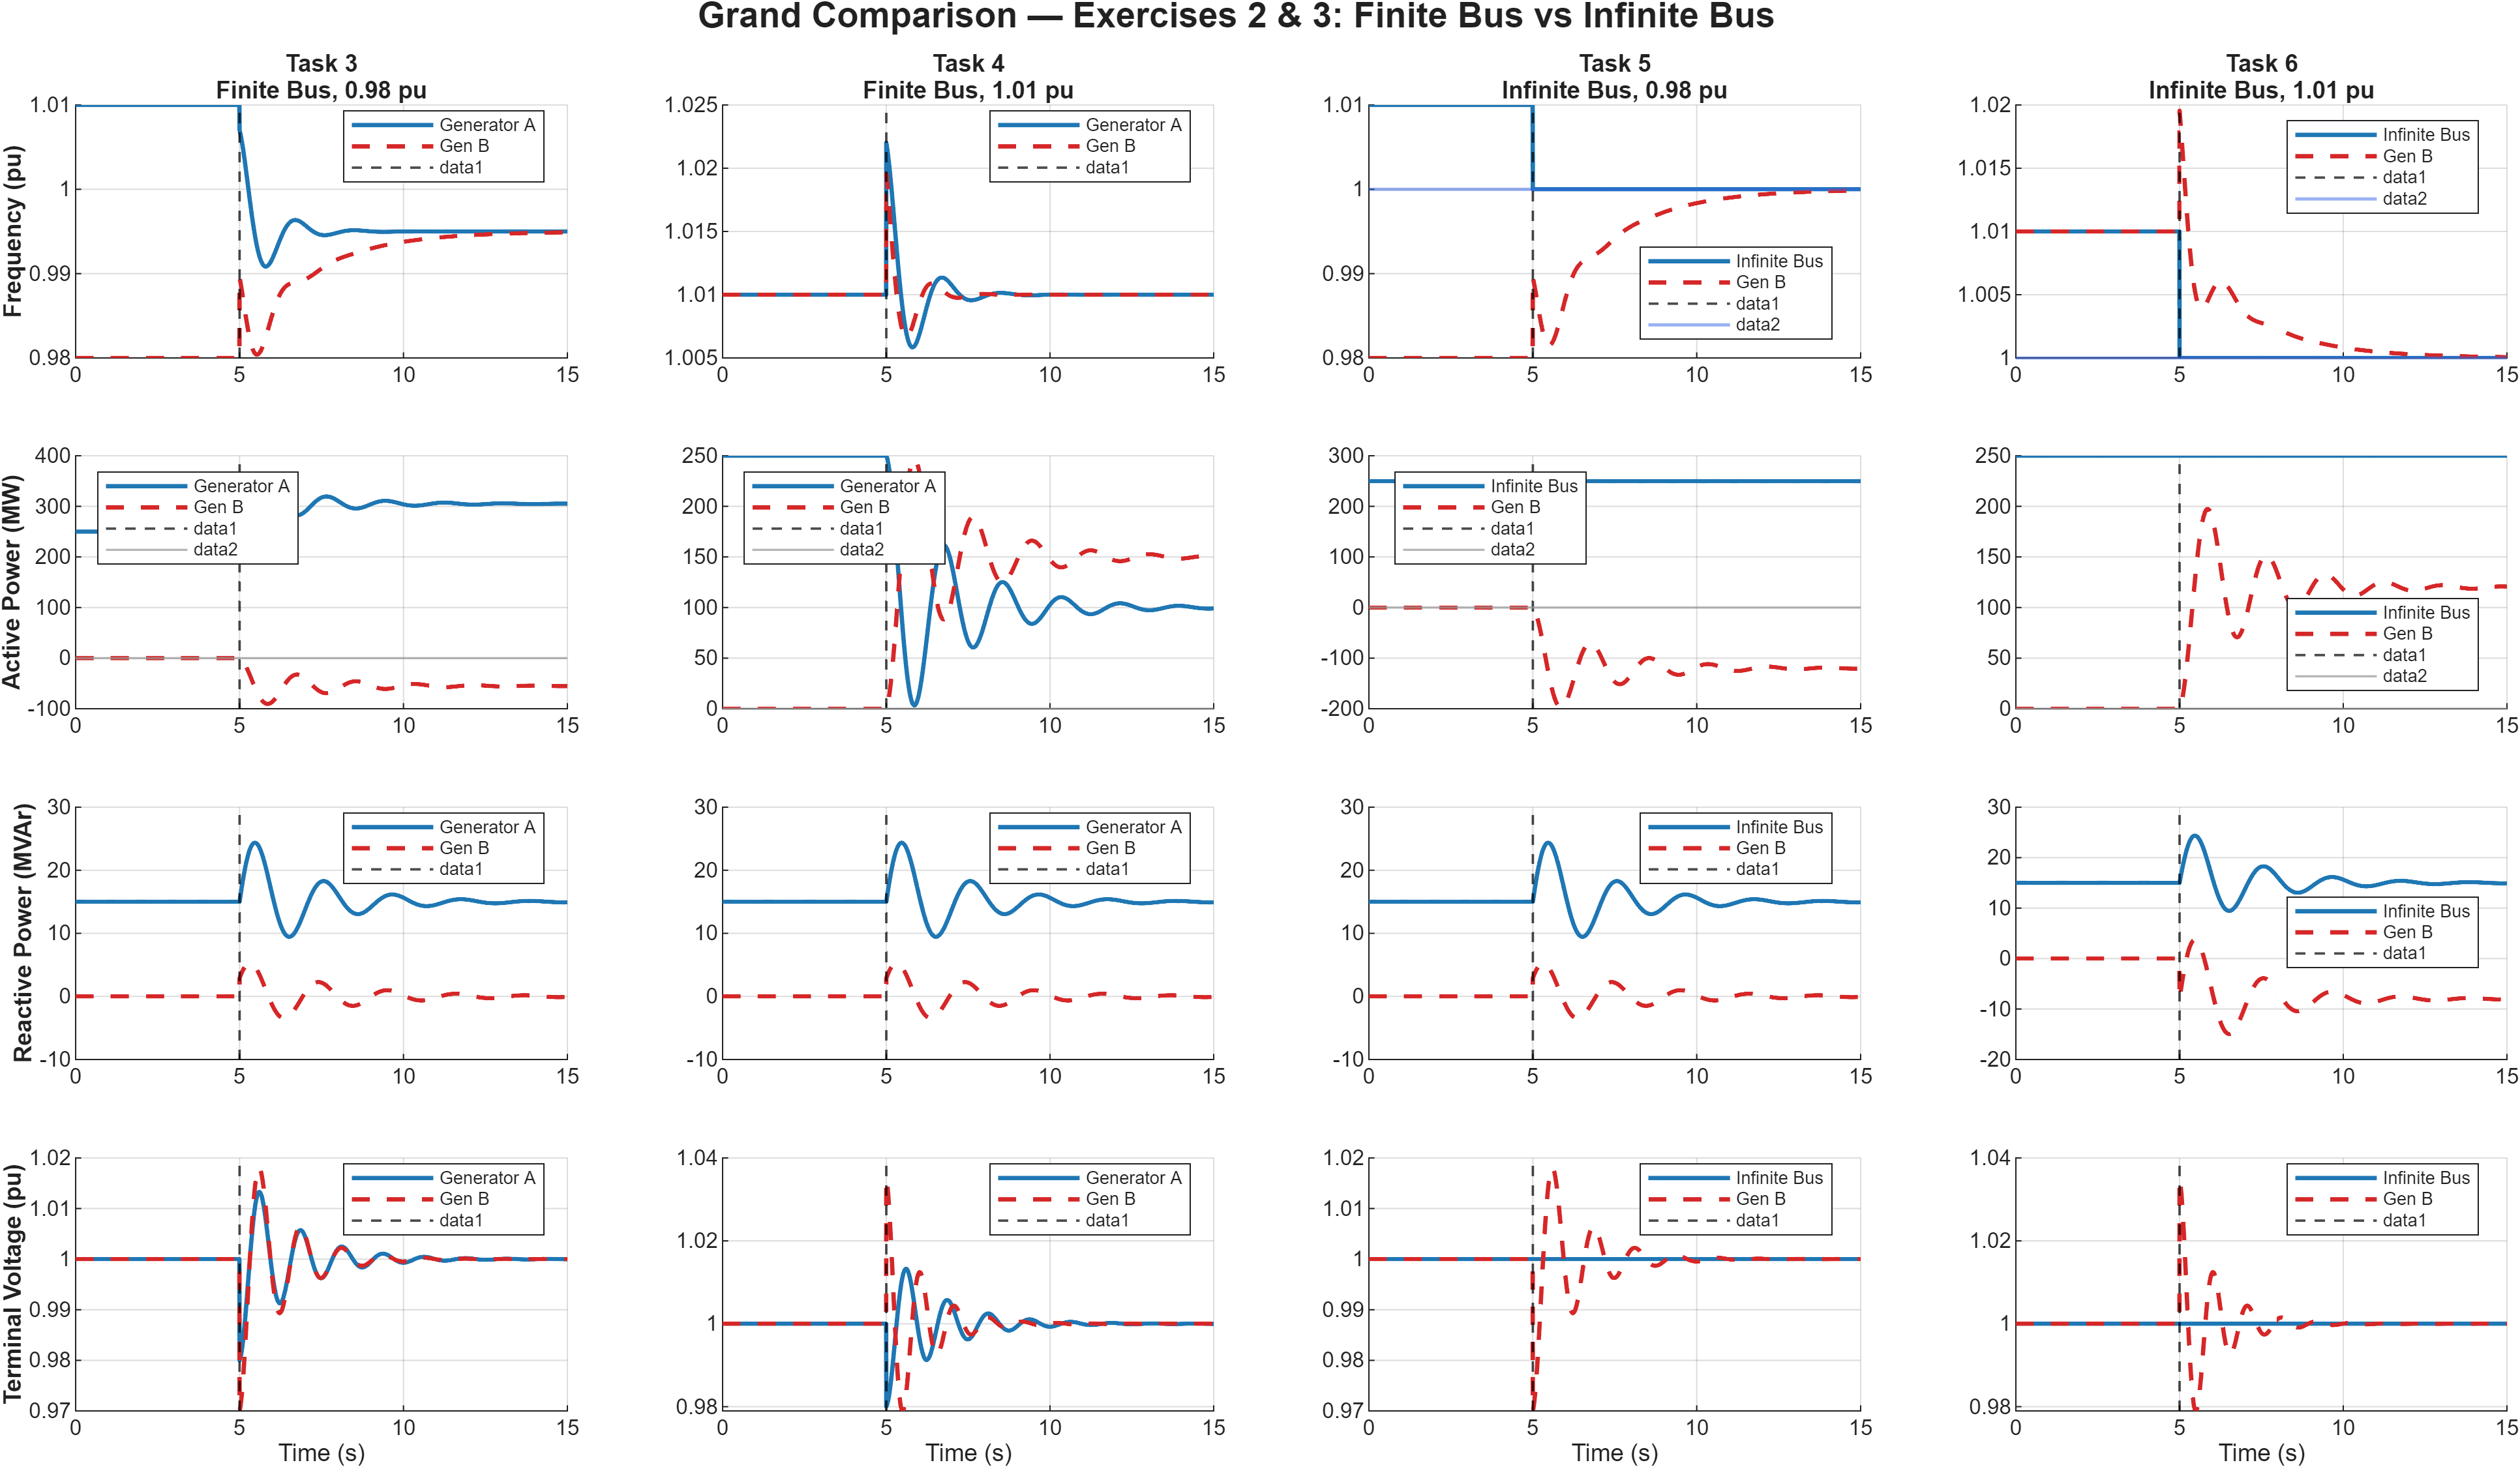
\includegraphics[width=\textwidth]{figures/Grand_Comparison_AllTasks.png}
  \caption{Grand comparison across Tasks~3--6. Rows compare finite bus (Ex~2)
    vs infinite bus (Ex~3); columns compare under-frequency ($f_\text{set}=\pu{0.98}$)
    vs over-frequency ($f_\text{set}=\pu{1.01}$) setpoints. The infinite bus
    eliminates all frequency compromise and amplifies power mismatch.}
  \label{fig:grand_comparison}
\end{figure}

Key observations from the grand comparison:
\begin{itemize}[leftmargin=2em]
  \item \textbf{Finite bus (Tasks~3,~4):} System frequency settles at a
    weighted compromise. Both generators influence the outcome.
  \item \textbf{Infinite bus (Tasks~5,~6):} System frequency is immovable at
    \pu{1.0}. Gen~B's power is determined entirely by its setpoint offset
    from the grid frequency.
  \item \textbf{Under-frequency setpoint (Tasks~3,~5):} Gen~B consistently
    motors; the infinite bus case (Task~5) produces more severe motoring.
  \item \textbf{Over-frequency setpoint (Tasks~4,~6):} Gen~B consistently
    generates; the infinite bus case (Task~6) produces a clean, stable power
    injection set by the droop equation alone.
\end{itemize}
